\documentclass[10.5pt, twocolumn]{article}

\usepackage[english]{babel}
\usepackage{graphicx}
\usepackage{imakeidx}
\usepackage{mathrsfs, amsmath}
\usepackage{systeme}
\usepackage{array}
\usepackage[utf8]{inputenc}
\usepackage{siunitx}
\usepackage{booktabs}
\usepackage{adjustbox}
\usepackage{geometry}
\geometry{a4paper,total={145mm,210mm}}
\usepackage{makecell}
\usepackage{afterpage}
\usepackage{listings}
\usepackage{subcaption}
\usepackage[toc,page]{appendix}
\usepackage[table]{xcolor}
\usepackage{pifont} % ding symbols
\usepackage{tikz}
\usepackage{changepage}
\usepackage{multirow} % multi row in tables
\usepackage{booktabs}
\usepackage{textcomp} % registered and copyright symbol
\usepackage{lscape} % vertical instead to horizontal
\usepackage{longtable} % for more page tables
\usepackage{eurosym}
\usepackage{lmodern}
\usepackage{amstext}
\usepackage{pdfpages} % import pdf pages
%\usepackage[hidelinks]{hyperref} % delete ugly hyperref borders of hyperlink
\usepackage{hyperref} % internal hyperlinks
\usepackage{titling} % titles
\usepackage{titlesec} % subtitles
\usepackage{blindtext} % for casual texts
\usepackage{dblfloatfix} % forces image at bottom in two-column files
\usepackage{gensymb} % standard unit of measurement
\usepackage{enumitem}

\DeclareRobustCommand{\officialeuro}{%
  \ifmmode\expandafter\text\fi
  {\fontencoding{U}\fontfamily{eurosym}\selectfont e}}



\makeindex[columns=2, title=Indice alfabetico, options= -s mystyle.ist, intoc]

\newcommand*{\Scale}[2][4]{\scalebox{#1}{\ensuremath{#2}}}
\renewcommand*\contentsname{Indice}
\newcommand*\NewPage{\newpage\null\thispagestyle{empty}\newpage}
\newcommand{\Virgolette}[1]{``#1''}
\newcommand*\circled[1]{\tikz[baseline=(char.base)]{
	\node[shape=circle,draw,inner sep=2pt] (char) {#1};}}
\newcommand{\tikzcircle}[2][red,fill=red]{\tikz[baseline=-0.5ex]\draw[#1,radius=#2] (0,0) circle ;}%command for draw text circle coloured
\def\changemargin#1#2{\list{}{\rightmargin#2\leftmargin#1}\item[]}
\let\endchangemargin=\endlist
\makeatletter
\let\originalpart=\part



\newcolumntype{C}[1]{>{\centering\arraybackslash}p{#1}}
\newcolumntype{L}[1]{>{\arraybackslash}p{#1}}
\newcolumntype{R}[1]{>{\raggedleft}p{#1}}
\newcolumntype{G}[1]{>{\centering\arraybackslash\columncolor{gray0}}p{#1}}

\definecolor{gray0}{gray}{0.9}
\definecolor{gray1}{gray}{0.7}
\definecolor{gray2}{gray}{0.4}

\lstset{
	literate = {α}{{$\alpha$}}1 {∆}{{$\Delta$}}1 {θ}{{$\theta$}}1 {η}{{$\eta$}}1 {→}{{$\rightarrow$}}1 {∂}{{$\partial$}}1, %tutti i simboli da usare come codice
	language = Mathematica % linguaggio
}
\hypersetup{
	citebordercolor=red
}


% ----- TITLE
\titleformat*{\section}{\Large\bfseries}
\title{
	\large{University of Trento}\\
	\normalsize{Master in Mechatronics Engineering}\\
	\vspace{0.2cm}
	\large{\textit{Modelling and Simulation of Mechatronics Systems}}\\
	\vspace{0.2cm}
	\Large{\textbf{Development, analysis and optimization of the performance of an innovative driving simulator}}\\
	\vspace{0.25cm}
	\hrule
	\vspace{0.2cm}
	\large{\textbf{Kinematics analysis}}\\	% Title
	\vspace{0.2cm}
	\hrule
}
\author{A. Comoretto \and J. Losi \and S. Valentini}
\date{\vspace{0.5cm}}
% ----- TITLE


\begin{document}
\maketitle

The kinematic analysis...

\section{Kinematics equations}
In this section the mechanism's behaviour is studied.
In Figure \ref{f:Top-View} is shown the top view of the mechanism.
\begin{figure}[h!]
	\centering
	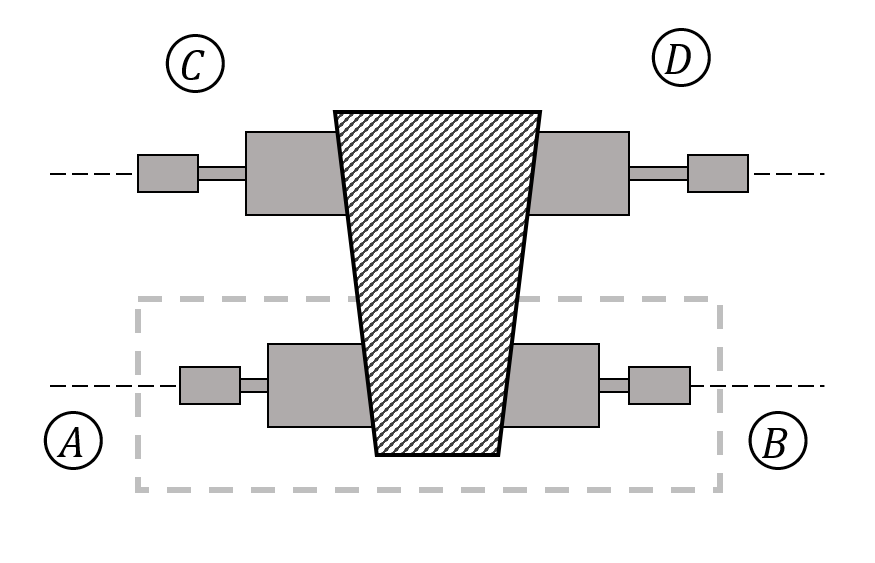
\includegraphics[width=7cm]{Images/Mechanism_TopView}
	\caption{Top view of the full-mechanism.}
	\label{f:Top-View}
\end{figure}

In first approximation a 2D analysis is conduced, and is refered only to the bodies \circled{A} and \circled{B}.

\subsection{2D-kinematics analysis}
The mechanism studied in the 2D simplification is the marked part in Figure \ref{f:Top-View}, in fact only bodies \circled{A} and \circled{B} are taken into account, and the result is shown in Figure \ref{f:2D_Mechanism}.
\begin{figure}[h!]
	\centering
	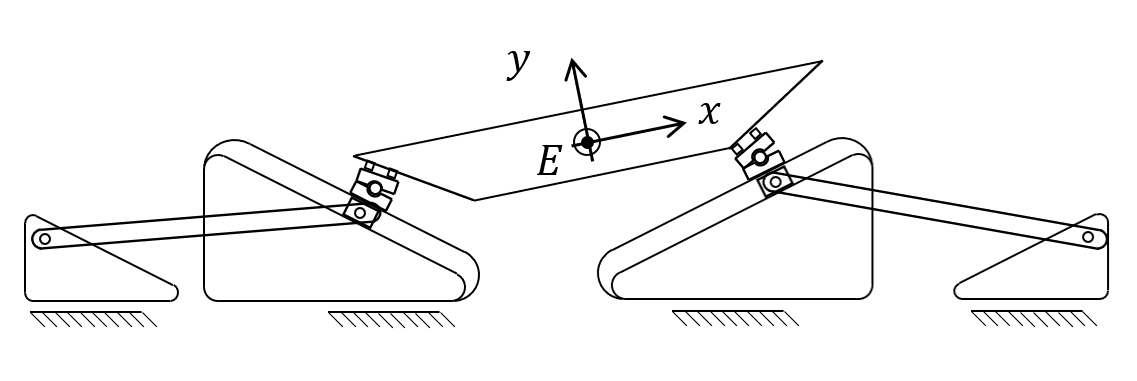
\includegraphics[width=7cm]{Images/Mechanism_LateralView}
	\caption{2D mechanism.}
	\label{f:2D_Mechanism}
\end{figure}

For the 2D analysis it is chosen to consider the length of the platform as a constant, even if it could be variable, due to its geometry.
More complex analysis are made in the following Section \ref{s:3D-kinematic} during the 3D analysis.

Thanks to this consideration it is possible to say that the full-mechanism is composed by two mirrored sub-mechanisms, made by four sub-bodies, joined by the platform.
So the sub-mechanism studied is shown in Figure \ref{f:Sub-Mechanism}.
\begin{figure*}[h!]
	\centering
	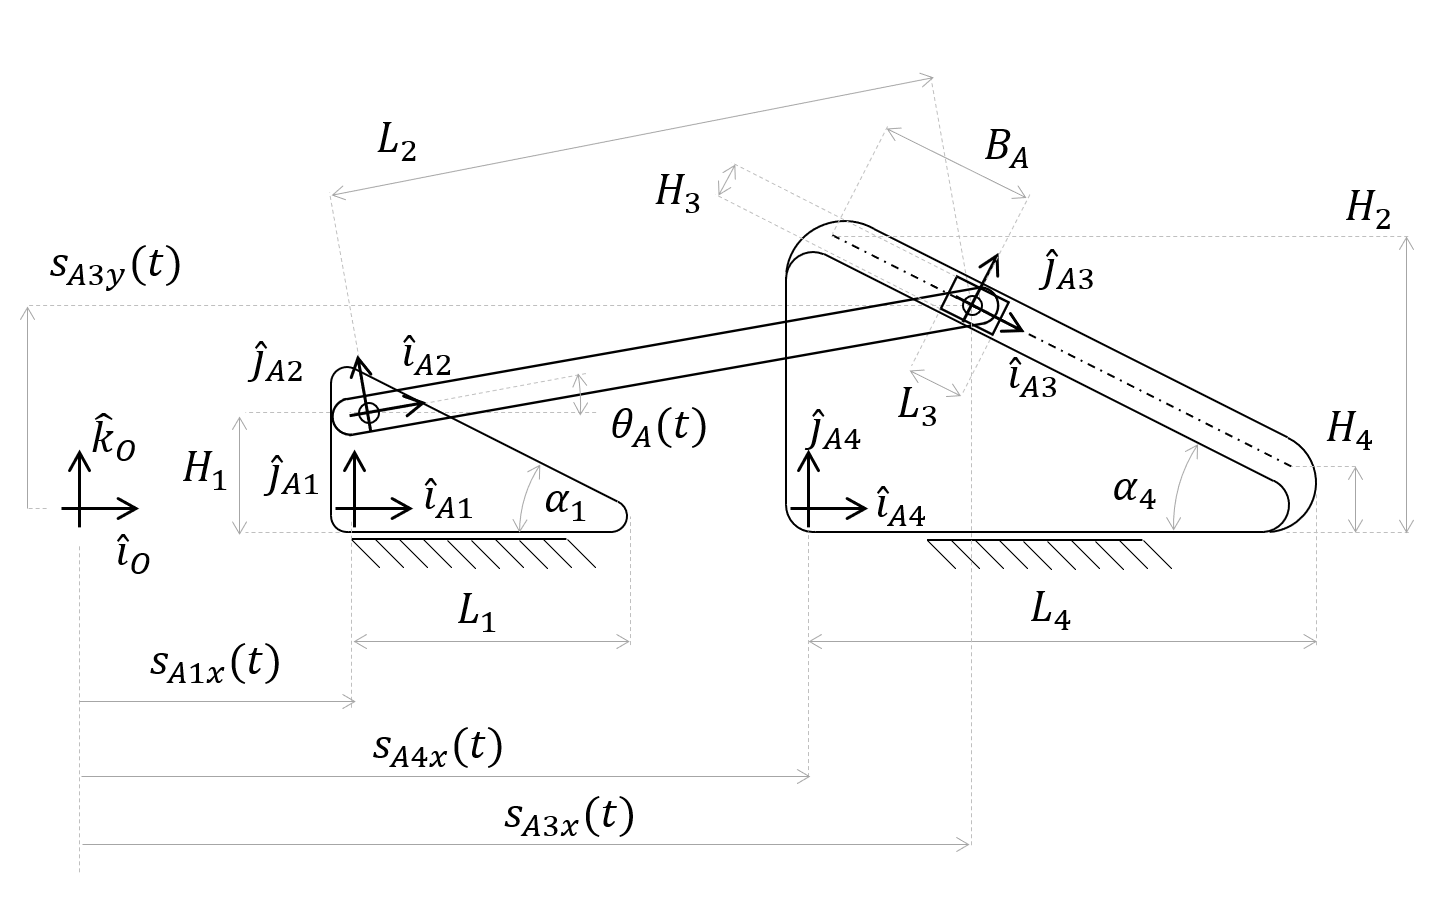
\includegraphics[width=12cm]{Images/Sub-Mechanism}
	\caption{One of the four sub-mechanism of the structure.}
	\label{f:Sub-Mechanism}
\end{figure*}
The same can be done for all the other sub-mechanisms by changing the subscripts.

At a first sight, it is easy to say that the four motors will be the independant variables, they are:
\begin{itemize}
  \item \( s_{A1x}(t) \);
  \item \( s_{A4x}(t) \);
  \item \( s_{B1x}(t) \);
  \item \( s_{B4x}(t) \).
\end{itemize}
Although the simplicity of this consideration it has to be revisited in way to work together with the previous one: in fact consider the length of the platform (named \( L_5\)) constant, means that one of the motor has to become a dependant variable.

In particular \( s_{A1x}(t) \) is considered the dependant variable.
\subsection{3D-kinematic analysis}
\label{s:3D-kinematic}

\section{Velocity analysis}

\section{Acceleration analysis}

\section{Effects of the main geometrical parameters}


\begin{thebibliography}{}
\bibitem{aVDS}
\Virgolette{\textit{Advanced Vehicle Driving Simulator}}, \textsc{ABDynamics}.

\bibitem{CKAS}
\Virgolette{\textit{6DOF Motion System}}, \textsc{CKAS}.

\bibitem{Kasim}
M. Kasim A. J., \Virgolette{\textit{Design and development of 6-dof motion platform for vehicle driving simulator}}, Universiti Teknologi Malaysia.
\end{thebibliography}
\end{document}
